\documentclass[]{auvsi_doc}
\setkeys{auvsi_doc.cls}{
	AUVSITitle={UGV Delivery System Selected Concept Description},
	AUVSIRevision=0.1,
	AUVSIDescription={Initial Draft},
	AUVSIAuthor={Kameron Eves},
	AUVSIChecker={????????},
	AUVSILogoPath={./figs/logo.pdf},
	AUVSIDocID={GV-005}
}

% include extra packages, if needed

% Remove Heading Numbers
\setcounter{secnumdepth}{0}

% Remove Heading Numbers
\setcounter{secnumdepth}{0}


% include extra packages, if needed

\begin{document}

\begin{AUVSITitlePage}
\begin{artifacttable}
\entry{GV-04, 1.0, 10-30-2018, Wrote concept description, Jacob Willis, CHECKED BY}
% additional \entry{} commands for extra rows in the revision table, if needed
\end{artifacttable}
\end{AUVSITitlePage}

% document contents (see below for LaTex commands that make your life easier)
\section{Introduction}
This document gives a more detailed description of the selected concept for the UGV delivery system. As can be seen from our selection matrix (GV-003) and test results (GV-004), the selected concept is a parachute with fins.

\section{Description}

The UGV will be loaded within the aircraft. Upon a command from the flight controller system small hatch will open and the UGV will fall out. Strings will attach the UGV to a lightweight fabric parachute. The fabric parachute will be loaded onto the aircraft in a tube that will allow the UGV to pull it out of the aircraft as it falls. This will help stop tangling that can come from a folded parachute. After exiting the aircraft the parachute will be opened by drag. The drag caused by the fabric will slow down the aircraft to a speed sufficient to allow the UGV to survive impact with the ground without damage. A visual depiction of our chosen system can be seen in Fig. \ref{fig:side}.

\begin{figure}[h]
\centering
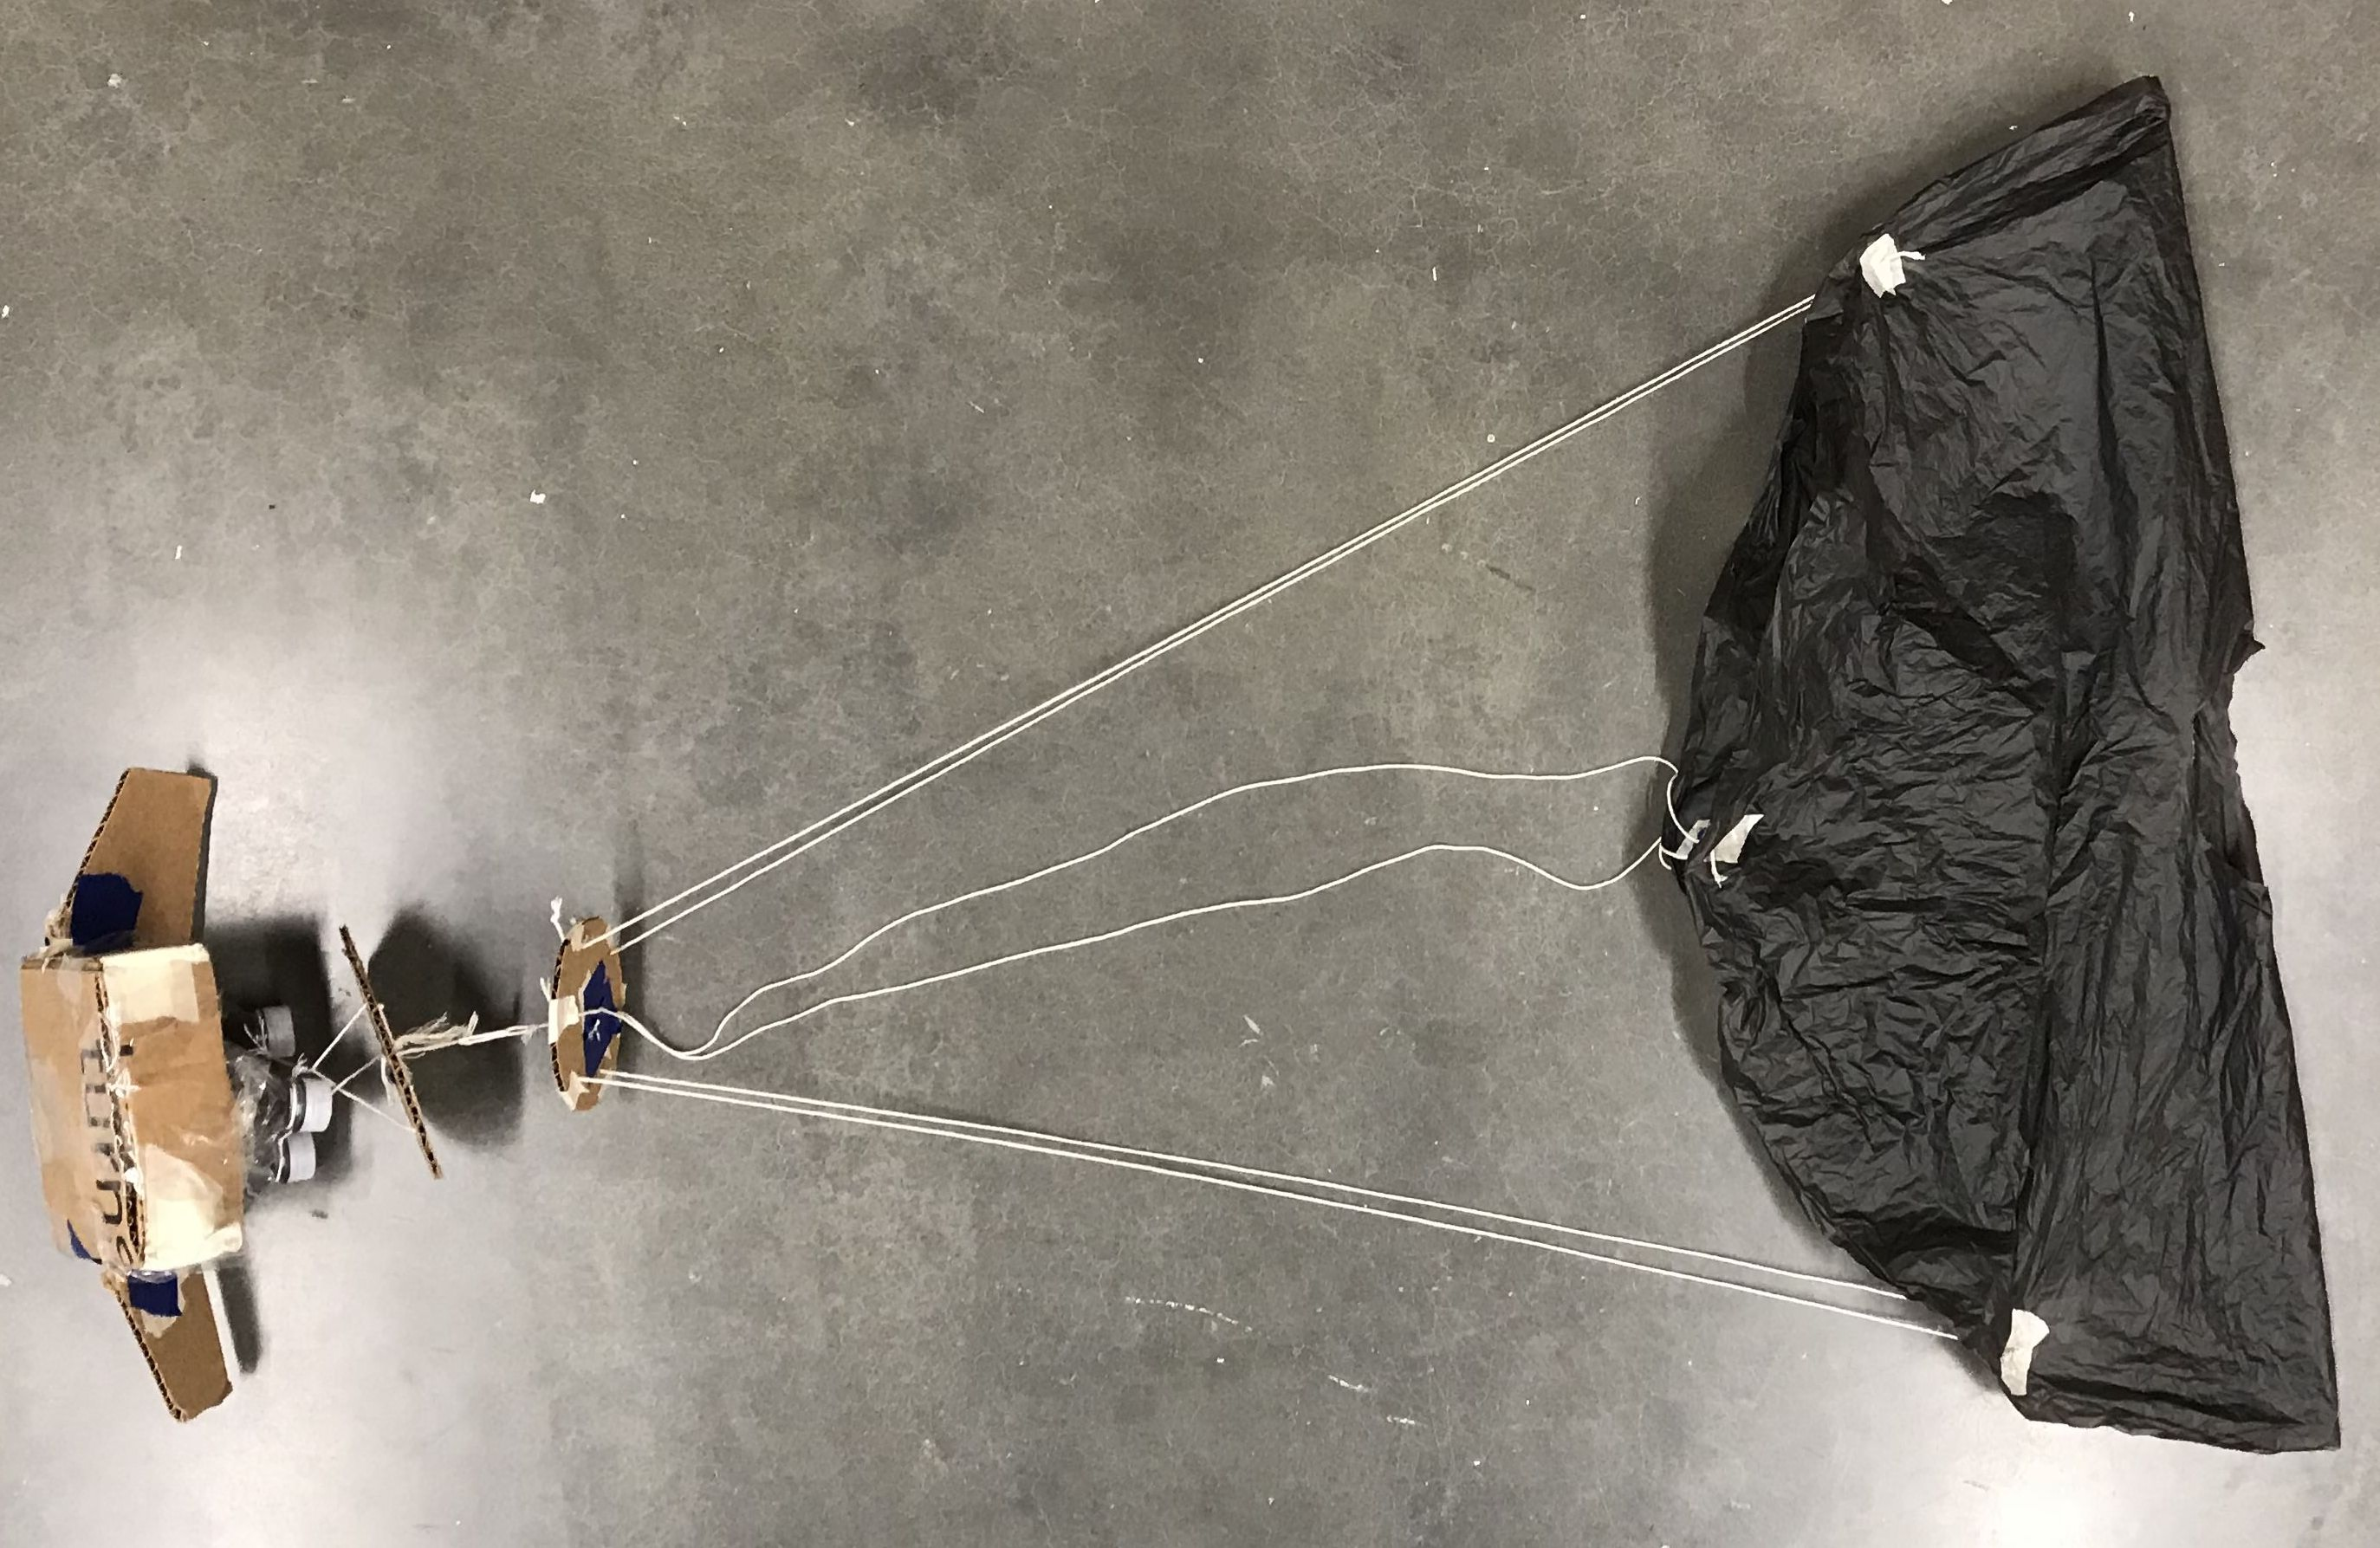
\includegraphics[width=90mm]{./figs/Parachute_Side.jpg}
\caption{A simple prototype of our parachute seen from the side.}
\label{fig:side}
\end{figure}

An accurate landing is another important part of the competition. A hole in the top of the parachute will improve the accuracy of the system. As can be seen in Fig. \ref{fig:top} we tested this hole in our prototype. This hole is known in the industry as a spill hole because it allows the air to spill out of the center of the parachute. This does increase the speed with which the system falls, but it also provides a market increase in the accuracy. This is because without the hole, the air become trapped within the system and excess air must move around the outside of the parachute as it falls through the air. Imperfections in manufacturing and weather conditions mean that this this overflow around the outside of the  parachute is always uneven. Thus the parachute is pushed to the side by the uneven overflow. A spill hole allows the overflow to "spill" out the top in a way that won't affect the lateral velocity of the system.

\begin{figure}[ht]
\centering
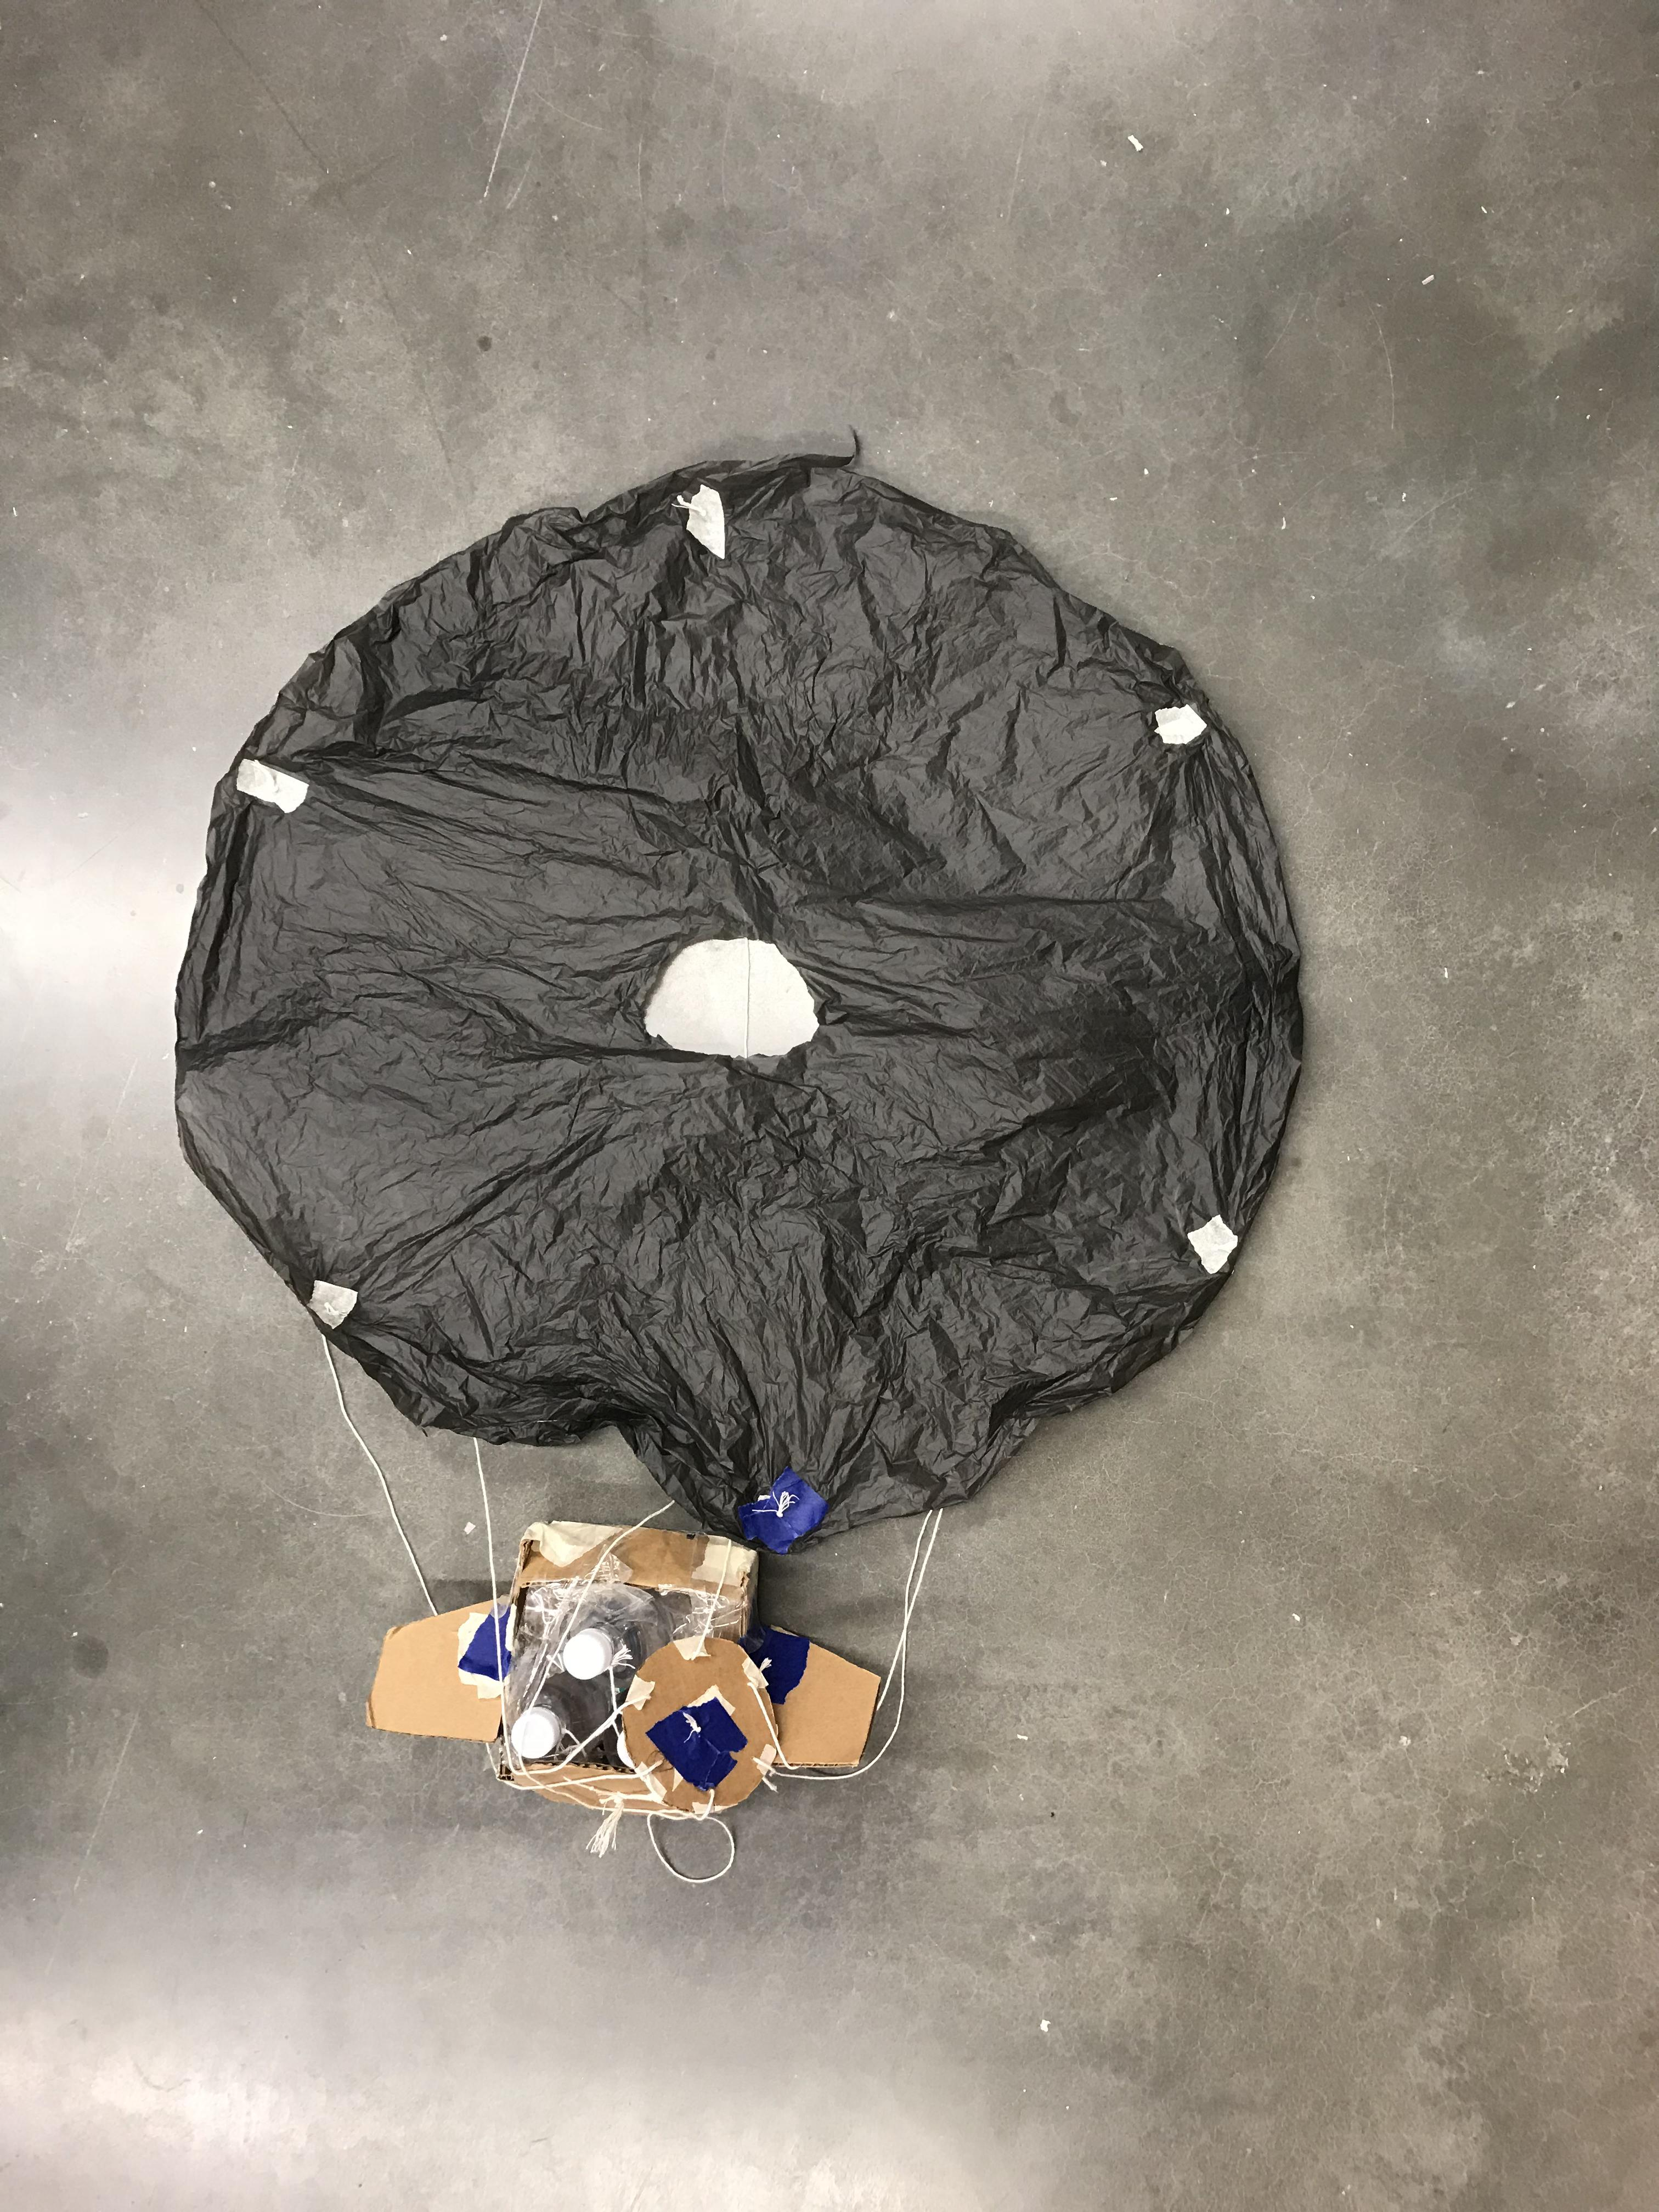
\includegraphics[width=90mm]{./figs/Parachute_Top.jpg}
\caption{A simple prototype of our parachute seen from the top. Note the hole in the middle of the parachute. As mentioned above, we found that this greatly improved the accuracy of the parachute.}
\label{fig:top}
\end{figure}

Fins are another way the accuracy of the system can be effected. These fins can be seen in one prototype in Fig.~\ref{fig:fins}. As can be seen in our testing results artifact (GV-004) the fins did push the system one direction. This should allow us to slightly control our system as it falls. While this will not be enough to correct for large errors, it should be enough to ensure we don't drift randomly. The protocol for dropping objects from a UGV, as detailed in \textit{Small Unmanned Aircraft: Theory and Practice} by Randy Beard and Tim McLain should also help improve our accuracy. This protocol uses the wind and velocity of the aircraft to predict the best location to release the payload.

\begin{figure}[ht]
\centering
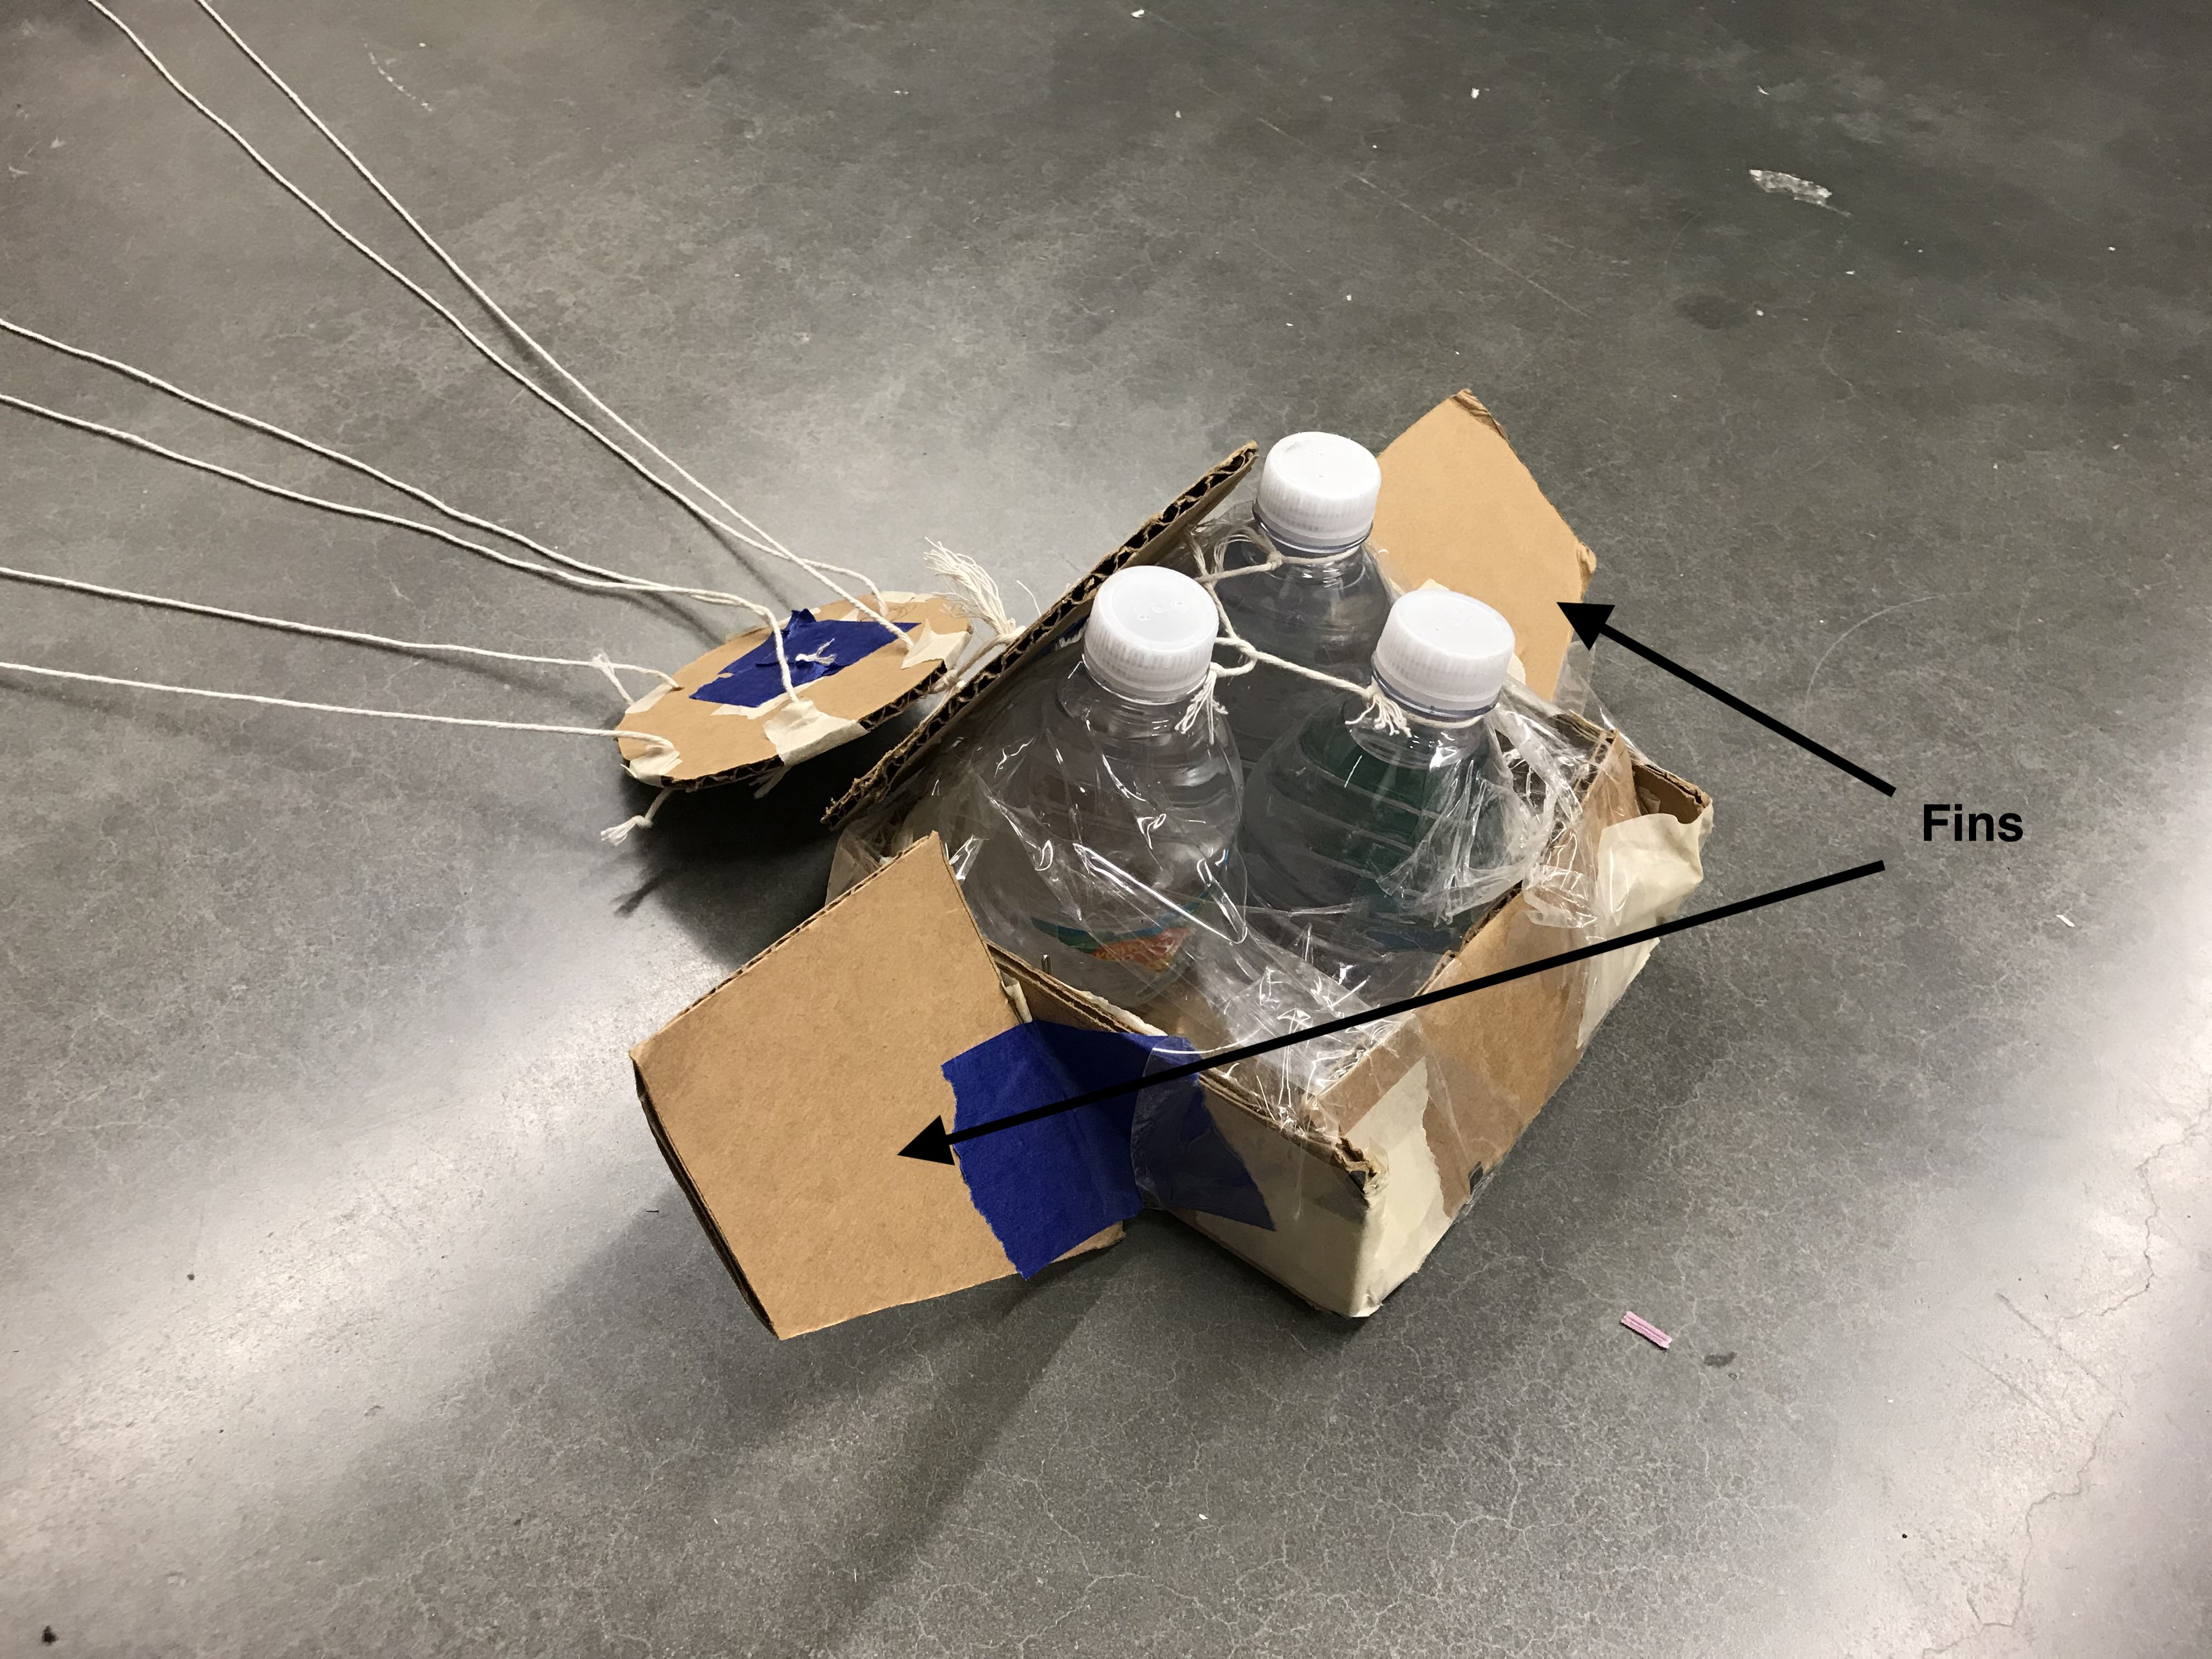
\includegraphics[width=90mm]{./figs/Parachute_Fins.jpg}
\caption{The payload we used to simulate the UGV. Note the fins. As mentioned above, preliminary results seem to indicate that these fins provided a small amount of control authority over the parachute's trajectory. This will help us improve accuracy}
\label{fig:fins}
\end{figure}

Using the system described above, we are confidant in our ability to achieve a landing accuracy of within 25 feet. This is considered excellent performance in our key success measures and will give us 75\% of the points possible in this portion of the competition. 

\end{document}
